\documentclass[11pt,a4paper,parskip=half ]{scrartcl}
\usepackage[utf8]{inputenc}
\usepackage[ngerman]{babel}
\usepackage{amsmath}
\usepackage{amsfonts}
\usepackage{amssymb}
\usepackage{graphicx}
\usepackage{xcolor}
\usepackage{float}
\usepackage{graphicx}
\usepackage{hyperref}

\author{Aaron Winziers - 1176638; Michael Wolz - 1195270}
\title{Digital Libraries WS 2018/2019\\\LARGE{Übungsblatt 1}}

\begin{document}
	\maketitle
	
	\section*{Aufgabe 1}
	
	\subsection*{a)}
	
	\begin{itemize}
		\item Das Schiff \glqq{}Titanic\grqq{}
		\item Den Film \glqq{}Titanic\grqq{}
		\item Den damit verbundenen Unfall mit dem Eisberg
	\end{itemize}
	
	\subsection*{b)}
	\begin{table}[H]
		\centering
		\begin{tabular}{|l|l|l|}
			\hline
			& Google & Yahoo \\ \hline
			Schiff   & 2      & 1     \\ \hline
			Film     & 2      & 7     \\ \hline
			Unfall   & 2      & 1     \\ \hline
			Sonstige & 3      & 1     \\ \hline
		\end{tabular}
	\end{table}
	Eine Zuordnung ist nicht immer eindeutig möglich, da in der Sprache oftmals
	eine Bezeichnung für mehrere Bedeutungen verwendet wird. 
	
	\subsection*{c)}
	Der Suchbegriff könnte erweitert werden, so dass das Informationsbedürfnis
	besser abgedeckt wird. So könnte der Suchbegriff dann z.B.  \glqq{}Titanic
	Schiff\grqq{}, \glqq{}Titanic Unfall\grqq{} oder \glqq{}Titanic Film\grqq{}
	lauten. 
	
	
	\section*{Aufgabe 2}
	
	\subsection*{a)}
	Welche Software gibt es, um eine digitale Bibliothek zu erstellen. \\
	Suchbegriff:  \glqq{}digital library software\grqq{}
	
	\begin{center}
		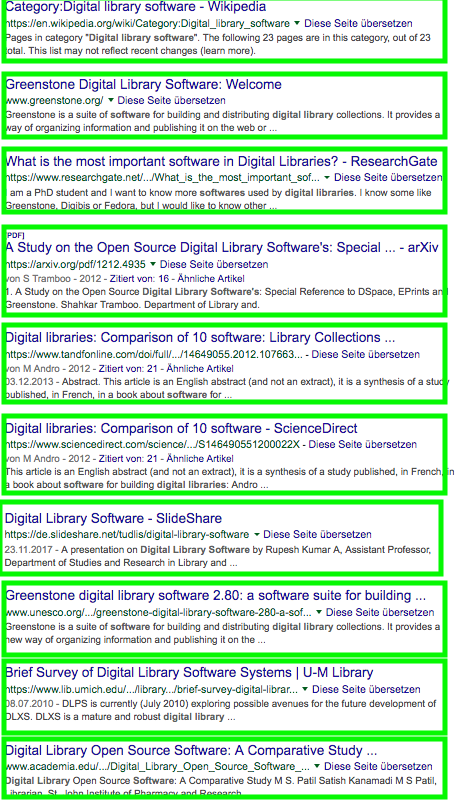
\includegraphics[height=0.8\textheight]{digital-libraries.png}
	\end{center}
	
	\subsection*{b)}
	Die relevanten Ergebnisse wurden in dem Screen in a) grün markiert. Es ergibt
	sich eine Präzision von 100\%. 
	
	\subsection*{c)}
	Für den Recall müssen alle Ergebnisse der Anfrage betrachtet werden. Da dies in
	unserem Fall bei Google \glqq{}ungefähr 568000000\grqq{} Ergebnisse sind, wäre
	es mit einem \textbf{extremen} Arbeitsaufwand verbunden, diese alle
	durchzugehen. Um den Recall von zwei Suchmaschinen zu vergleichen,d könnte man
	die relevante Menge z.B. auf die ersten 100 Ergebnisse einschränken.
	
	\section*{Aufgabe 3}
	\subsection*{a)}
	\subsubsection*{F-Measure} Seien R der Recall und P die Precision dann ist
	\begin{center}
		$F_{\beta}=(1+\beta^{2})\cdot\frac{P\cdot R}{(\beta^{2}\cdot P)+R}$
	\end{center}
	Dabei gibt $\beta$ an wie Recall und Precision gewichtet werden sollen. Bei
	$\beta>1$ wird Precision höher gewichtet, bei $0<\beta<1$ wird Recall höher
	gewichtet. Das F-Measure ist ein Evaluationsmaß, das Precision und Recall eines
	Systems verrechnet.
	\begin{itemize}
		\item $F_{\beta}=0$ kann dann vorkommen, wenn Precision oder Recall = 0, d.h.
		wenn keine relevante Ergebnisse geliefert werden.
		\item $F_{\beta}=1$ kann dann vorkommen, wenn alle relevante Ergebnisse
		geliefert werden (Recall = 1) und alle Ergebnisse relevant sind (Precision = 1)
	\end{itemize}
	
	\subsubsection*{Fallout} Sei FP die Menge der False-Positives oder die Menge
	der gelieferten Ergebnisse die nicht relevant sind und TN die Menge der
	True-Negatives, oder die Menge der nicht relevanten Daten die tatsächlich nicht
	in der Ergebnismenge liegen, dann
	\begin{center}
		$Fall-out = \frac{FP}{FP+TP}$
	\end{center}
	\begin{itemize}
		\item \textbf{Fallout = 0} kommt vor, wenn alle Ergebnisse relevant sind
		\item \textbf{Fallout = 1} kommt vor, wenn alle Ergebnisse \textit{nicht}
		relevant sind 
	\end{itemize}
	
	\textit{Quelle:}\url{https://www.wikipedia.com/en/Precision_and_recall}
	
	\subsection*{b)}
	\begin{itemize}
		\item[TP](True-Positives) - Die Menge der relevante Ergebnisse
		\item[TN](True-Negatives) - Die Menge der nicht relevante Daten die nicht in
		der Ergebnismenge geliefert werden
		\item[FP](False-Positives) - Die Menge der nicht relevante Ergebnisse
		\item[FN](False-Negatives) - Die Menge der relevante Daten die nicht in der
		Ergebnismenge geliefert werden
	\end{itemize}
	\textbf{Relevante Menge:}$\{d_{1}, d_{4}, d_{5}, d_{6}, d_{9}, d_{13}, d_{17},
	d_{18}, d_{26}\}$  = 9	\\
	
	\textbf{$S_{1}$:}$\{d_{1},d_{3},d_{6},d_{7},d_{9},d_{13},d_{15},d_{16},d_{17},d_{24}\}$
	\\
	TP = 5, FN = 4, FP = 4, TN = 17
	\begin{itemize}
		\item Recall = $\frac{5}{5+4} = \frac{5}{9}$
		\item Precision = $\frac{5}{5+4} = \frac{5}{9}$
		\item Fall-out = $\frac{4}{4+17} = \frac{4}{21}$
		\item $F_{1}$ = $\frac{2\cdot5}{2\cdot5+4+4} = \frac{5}{9}$
	\end{itemize}
	
	
	\textbf{$S_{2}$:}$\{d_{2},d_{5},d_{6},d_{9},d_{10},d_{13},d_{17},d_{18},d_{21},d_{22},d_{24},d_{26},d_{27}\}$
	\\ 
	TP = 7, FN = 2, FP = 6, TN = 15
	\begin{itemize}
		\item Recall = $\frac{7}{7+2} = \frac{7}{9}$
		\item Precision = $\frac{7}{7+6} = \frac{7}{13}$
		\item Fall-out = $\frac{6}{6+15} = \frac{6}{21}$
		\item $F_{1}$ = $\frac{2\cdot7}{2\cdot7+6+2} = \frac{7}{11}$
	\end{itemize}
	
	\textbf{$S_{3}$:}$\{d_{1},d_{3},d_{6},d_{10},d_{13},d_{17},d_{18},d_{26}\}$	\\
	TP = 6, FN = 3, FP = 2, TN = 19
	\begin{itemize}
		\item Recall = $\frac{6}{6+3} = \frac{2}{3}$
		\item Precision = $\frac{6}{6+2} = \frac{3}{4}$
		\item Fall-out = $\frac{2}{2+19} = \frac{2}{21}$
		\item $F_{1}$ = $\frac{2\cdot6}{2\cdot6+2+3} = \frac{2}{3}$
	\end{itemize}
	
	Je nachdem welches Maß man als am sinnvollsten sieht sind Verschiedene Resultate das "Beste". Nach dem Recall hat $S_{2}$ das beste Ergebnis geliefert, nach Precision, $F_{1}$ und Fall-out war $S_{3}$ das beste Resultat.
	\subsection*{c)}
	Um Recall = 1 zu erreichen geben wir alle Dokumente zurück
	\begin{itemize}
		\item Precision: Gleich der prozentualen Menge der Relevanten Ergebnisse
		\item Fallout: 1, da alle nicht relevante Daten in der Ergebnismenge enthalten sind
		\item $F_{1}$: Abhängig davon wie groß die Menge der tatsächlich relevanten Ergebnisse ist im Verhältnis zu der der nicht relevanten
	\end{itemize}
	
	Um Fall-out = 0 zu erreichen geben wir keine Dokumente zurück
	\begin{itemize}
		\item Precision: Nicht definiert wegen Division von 0
		\item Recall: 0, da es keine True-Positives gibt
		\item $F_{1}$: 0, da es keine True-Positives gibt
	\end{itemize}
	
	Der Korpus muss mindestens ein Dokument beinhalten.
	
	
\end{document}
